%% ------------------------------------------------------------------------------------------- Results
\section{Results}
\label{sec:results}

\begin{table*}[t]
\centering
\small
\setlength{\tabcolsep}{6pt}
\begin{tabular}{lccccc}
\toprule
Pipeline & Normal & Low light & Far (2$\times$) & Crowded & All \\
\midrule
Baseline (full frame) & 91.0 & 67.0 & 63.6 & 70.0 & 72.9 \\
Ours, $s{=}3$ (proposal) & 67.8 {\scriptsize($-$23.2$^\dagger$)} & 47.2 {\scriptsize($-$19.8$^\dagger$)} & 64.6 {\scriptsize(+1.0)} & 66.8 {\scriptsize($-$3.2)} & 61.6 {\scriptsize($-$11.3$^\dagger$)} \\
Ours, $s^*{=}6$, SCRFD (val-sel.) & 93.8 {\scriptsize(+2.8$^\dagger$)} & 77.0 {\scriptsize(+10.0$^\dagger$)} & 94.0 {\scriptsize(+30.4$^\dagger$)} & 77.4 {\scriptsize(+7.4$^\dagger$)} & 85.5 {\scriptsize(+12.7$^\dagger$)} \\
\bottomrule
\end{tabular}
\vspace{-1mm}
\caption{\textbf{Main comparison} on the 100 held-out HaGRID subjects. Top-1 gesture accuracy (\%), with the paired change vs.\ the baseline in pp; $^\dagger$: exact McNemar $p<0.05$. Both pipelines use the \emph{same} pretrained MediaPipe Gesture Recognizer, scored on its 5 classes (2,000 images, 500 per condition). 95\% bootstrap CIs of the overall change are given in the text.}
\label{tab:main}
\vspace{-2mm}
\end{table*}

\noindent\textbf{Main comparison} (\cref{tab:main}). The \emph{pre-registered} cascade ($s{=}3$, BlazeFace)
is worse than the baseline: \mpSAllD\,pp overall (95\% CI [\mpSAllLo, \mpSAllHi]) and \mpSNorD\,pp on normal
images. It breaks \mpSAllBrk{} images and fixes only \mpSAllFix. With this setting \textbf{H1 is rejected}. The
setting \emph{selected on val} ($s^*{=}\mpTScale$, SCRFD anchor; val accuracy \mpValSSixscrfd\% vs.\
\mpValfull\% for the full frame) raises test accuracy from \mpBaseAllAcc\% to \mpTAllAcc\%, a gain of
\mpTAllD\,pp (CI [\mpTAllLo, \mpTAllHi], McNemar $p\mpTAllP$; \mpTAllFix{} fixed vs.\ \mpTAllBrk{} broken). It
improves every condition: \mpTFarD\,pp far, \mpTLowD\,pp low light, \mpTCroD\,pp crowded, and \mpTNorD\,pp normal
($p{=}\mpTNorP$). The gain comes from where the hand is small or degraded, as hypothesised, and the extra median
latency is \latExtramediapipe\,ms (\cref{tab:cost}). With the val-selected setting, \textbf{H1 is supported}.
Note, however, that this is not the setting we fixed in advance.

\begin{table}[t]
\centering
\footnotesize
\setlength{\tabcolsep}{2.6pt}
\begin{tabular}{lcccc}
\toprule
 & \multicolumn{4}{c}{MediaPipe} \\
\cmidrule(lr){2-5}
 & \multicolumn{2}{c}{BlazeFace} & \multicolumn{2}{c}{SCRFD} \\
$s$ & all & far & all & far \\
\midrule
full frame & \multicolumn{4}{c}{72.9 / 63.6} \\
\midrule
2 & 41.1 & 63.2 & 2.5 & 3.0 \\
3 (prop.) & 61.6 & 64.6 & 26.1 & 29.4 \\
4 & 73.1 & 64.4 & 66.0 & 72.6 \\
5 & 74.6 & 64.2 & 83.1 & 90.6 \\
6 & 74.6 & 64.2 & \textbf{85.5} & \textbf{94.0} \\
\midrule
3, no up-scale & 62.8 & 64.8 &  &  \\
3, shift $0.5h_f$ & 62.2 & 64.6 &  &  \\
\midrule
face found & 71.2 & 13.7 & 99.7 & 99.0 \\
\bottomrule
\end{tabular}
\vspace{-1mm}
\caption{\textbf{Ablation}: top-1 accuracy (\%) on all 4 conditions / far only, by ROI scale $s$ and face anchor; every cell uses the same detector weights and images. Bold: the configuration selected on the val split. ``face found'': \% of normal / far images in which the anchor found a face (otherwise the pipeline falls back to the full frame).}
\label{tab:abl}
\vspace{-3mm}
\end{table}

\noindent\textbf{Ablation} (\cref{tab:abl}). \emph{ROI size} matters most. HaGRID subjects hold the hand beside
the head, often more than one face-width away, so $s{\le}3$ cuts it off and accuracy falls far below the
baseline. It rises up to $s{=}6$, the edge of our grid, so a larger $s$ could be better still.
The \emph{anchor} decides the far condition. BlazeFace short-range finds a face in only \mpFaceSThreeUpnormal\% of
normal and \mpFaceSThreeUpfar\% of far images, and otherwise falls back to the full frame, so BlazeFace ROIs
cannot beat the baseline on far images. SCRFD finds a face in $\geq$98\% of the images in every condition.
SCRFD boxes are tighter, so SCRFD needs $s{\ge}5$, but at that size it lifts far accuracy to
\mpAccFarSSixUpScrfd\%.
\emph{Up-scaling} and \emph{shifting the ROI} down by half a face change accuracy by ${\approx}1$\,pp at $s{=}3$.

\begin{table}[t]
\centering
\footnotesize
\setlength{\tabcolsep}{4pt}
\begin{tabular}{lccc}
\toprule
Pipeline & median & p95 & extra \\
\midrule
full frame & 15.6 & 22.2 & -- \\
ROI $s{=}3$, BlazeFace & 17.4 & 24.3 & +1.8 \\
ROI $s{=}6$, SCRFD & 22.1 & 28.7 & +6.4 \\
\midrule
SCRFD + ArcFace (both) & 10.0 & 18.9 & -- \\
\bottomrule
\end{tabular}
\vspace{-1mm}
\caption{\textbf{Cost}: CPU latency per selfie in ms (100 native-resolution test images, cpu, Ryzen 7 7800X3D, decode excluded). The ROI pipeline includes the anchor face detector and the crop, and makes one face-detector call plus one gesture-detector call per image. Model sizes: MediaPipe GR 8.0\,MB, BlazeFace 0.22\,MB, SCRFD 2.4\,MB, ArcFace 13.0\,MB.}
\label{tab:cost}
\vspace{-3mm}
\end{table}
\begin{table}[t]
\centering
\footnotesize
\setlength{\tabcolsep}{2.2pt}
\begin{tabular}{lccccc}
\toprule
Pipeline & FRR & FAR$_\text{bg}$ & FAR$_\text{face}$ & FAR$_\text{gest}$ & FAR$_\text{rep}$ \\
\midrule
full & 30.1 & 13.6 & 0.65 & 0.95 & 45.2 \\
ROI $s{=}3$, BlazeFace & 40.4 & 7.1 & 0.58 & 0.70 & 36.7 \\
ROI $s{=}6$, SCRFD & 15.3 & 0.8 & 0.75 & 0.21 & 46.5 \\
\bottomrule
\end{tabular}
\vspace{-1mm}
\caption{\textbf{End-to-end} accept/reject (\%; gesture \emph{and} ArcFace, $\tau{=}0.2235$). FRR: genuine check-ins rejected (all conditions). FAR$_\text{bg}$: the challenge is the gesture of the \emph{other} person in a crowded image. FAR$_\text{face}$: another enrolled student's identity is claimed. FAR$_\text{gest}$: a wrong gesture is accepted. FAR$_\text{rep}$: an old photo passes a random challenge within 3 attempts.}
\label{tab:sec}
\vspace{-3mm}
\end{table}

\noindent\textbf{Cost} (\cref{tab:cost}). Both pipelines make one gesture-detector call. The cascade adds one
face-detector call and a crop. With SCRFD the face detection can be shared with the identity branch, which runs
SCRFD anyway, so in a deployed system the added cost is close to zero.

\noindent\textbf{End to end} (\cref{tab:sec}). With face verification included, the val-selected cascade halves
the false-reject rate (\mpFRRFull\%$\rightarrow$\mpFRRRoiSix\%; far: \mpFRRFullfar\%$\rightarrow$\mpFRRRoiSixfar\%).
It also blocks the background-hand attack (\mpFARbgFull\%$\rightarrow$\mpFARbgRoiSix\%). With the ROI, the gesture
and the verified face come from the same person: an attacker who copies a classmate's gesture is matched against
the face next to that hand, and that face is not theirs. Impostor-face FAR stays below 1\%. On LFW-calibrated
ArcFace, normal images give FRR \faceFRRnormal\% and FAR \faceFARnormal\%.

\begin{figure*}[t]
  \centering
  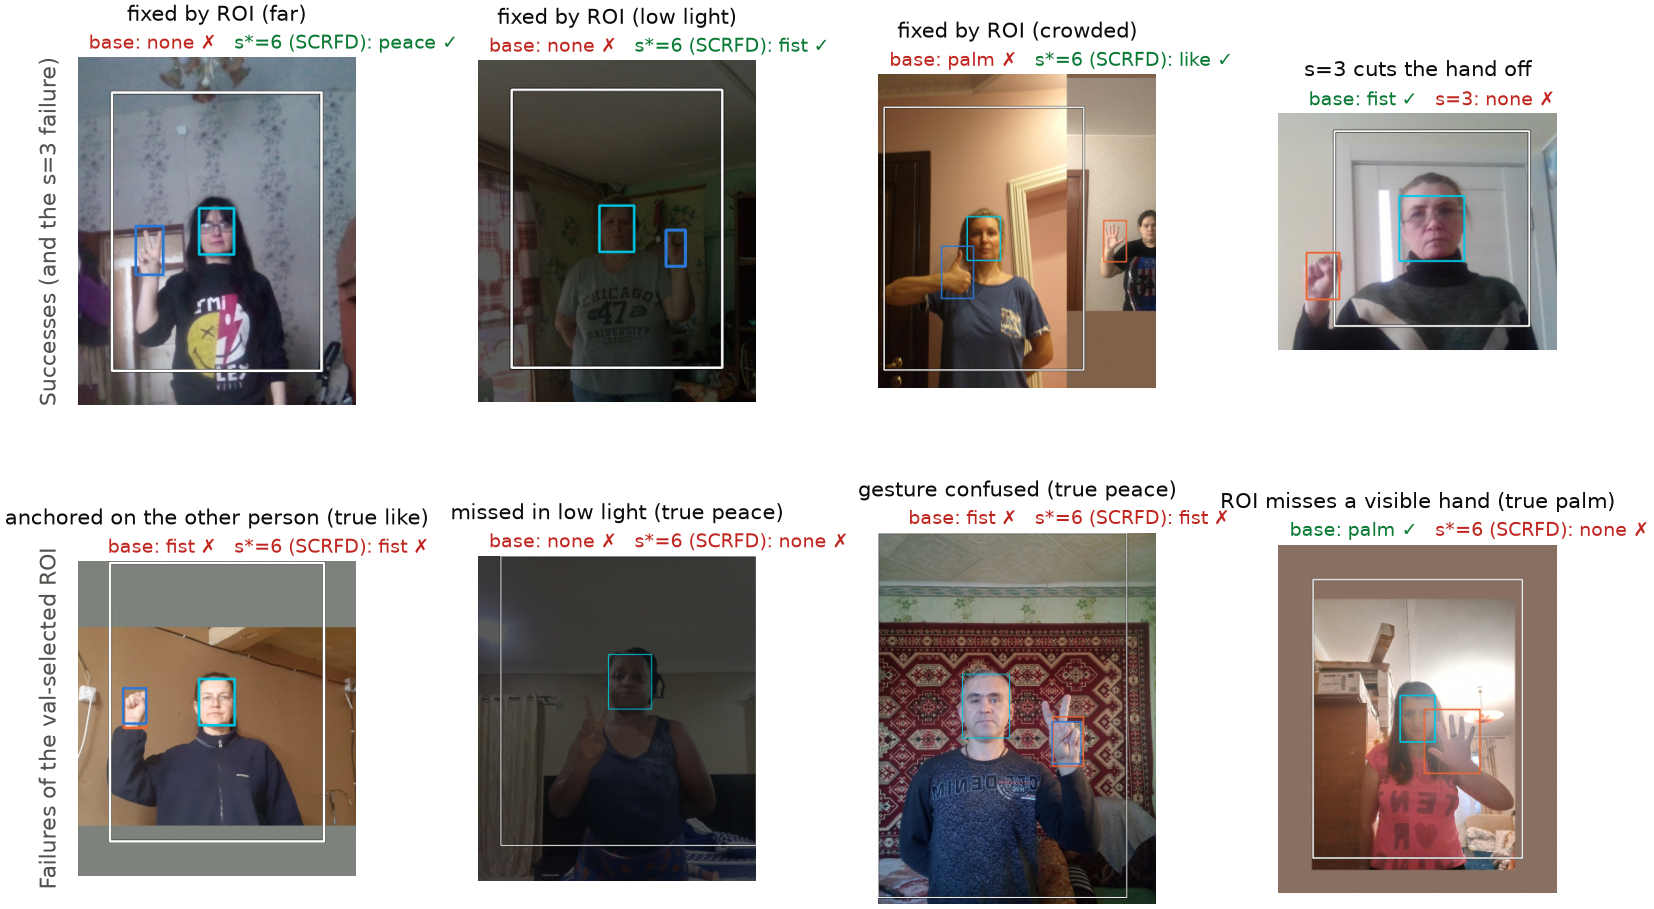
\includegraphics[width=0.8\linewidth]{figures/qualitative.png}
  \vspace{-1.5mm}
  \caption{\textbf{Qualitative examples} (held-out test images, zoomed). White: ROI; cyan: anchor face;
  orange: baseline's top detection; blue: ours. Top: successes of the val-selected ROI and the typical failure of
  the proposal's $s{=}3$. Bottom: failures of the val-selected ROI.}
  \label{fig:qual}
  \vspace{-3mm}
\end{figure*}

%% ------------------------------------------------------------------------------------------- Failures
\section{Failure analysis and limitations}
\label{sec:fail}

\noindent\textbf{Where it fails} (\cref{fig:qual}, bottom). Of the \mpTErrErrors{} errors of the val-selected
cascade, \mpTErrNoDetectionInRoi{} are hands that MediaPipe misses inside the ROI. These are mostly in low light
(\mpTErrErrorsLowLight{} errors) and in crowded images (\mpTErrErrorsCrowded). \mpTErrWrongClass{} are wrong
classes and only \mpTErrNoFaceFound{} have no face. \mpTErrBaselineAlsoWrong{} of the \mpTErrErrors{} errors are also
made by the baseline. (1)~\emph{Wrong anchor}: the ``largest face'' rule picks the background person in
\mpWrongAnchorSSixUpScrfd\% of crowded images, because that person's face can be bigger in pixels. The genuine
student is then rejected; the attack still fails, since the face does not match. (2)~\emph{ROI too small}: the
proposal's $s{=}3$ cuts off hands held at arm's length (top right). The ROI size is a property of how users pose,
so it must be validated on the target population. (3)~\emph{Replay}: a stored photo passes a random 1-of-5
challenge within 3 attempts 36.7--46.5\% of the time, whichever pipeline is used. The gesture challenge alone is weak liveness;
two-gesture challenges or fewer attempts are needed.

\noindent\textbf{Bias.} On HaGRID's automatic labels (aggregated per subject), the val-selected cascade scores
\mpBiasTgenderfemale\% for female and \mpBiasTgendermale\% for male subjects, and \mpBiasTagegroupYoung\% for
subjects under 25 vs.\ \mpBiasTagegroupOld\% for those over 40. This narrows the baseline's age gap
(\mpBiasFullagegroupYoung\% vs.\ \mpBiasFullagegroupOld\%). Only \mpBiasNraceBlack{} Black, \mpBiasNraceAsian{} Asian
and \mpBiasNraceIndian{} Indian subjects are in the test set, too few for conclusions about race. Face verification
bias was not measured per group.

\noindent\textbf{Limitations.} The far, low-light and crowded conditions are \emph{synthetic}: real distance also
blurs the image and real low light changes the noise. We did not collect the planned classroom volunteer set, so
there are no real phone selfies from our own population; this is the most important missing evidence. HaGRID
subjects are 80\% White. The tested scales stop at the grid edge. Only one gesture detector was evaluated.
InsightFace weights are licensed for non-commercial research only, and storing face embeddings needs consent and a
deletion policy. The app keeps only embeddings and lets the instructor delete them.
